\documentclass{beamer}
\usepackage{amsfonts,amsmath}
\usetheme{-statale}
\usefonttheme[onlymath]{serif}

\usepackage[italian]{babel}
\usepackage{bussproofs}
\usepackage{tabularx}
\usepackage{multirow}
\usepackage{tabularray}

\usepackage{float}
\usepackage{subcaption}
\usepackage{tikz}
\usetikzlibrary{positioning}
\usepackage{stmaryrd}
\usepackage{subcaption}
\usepackage{caption}
\usepackage{siunitx}

\EnableBpAbbreviations

\newcommand{\testcolor}[1]{\colorbox{#1}{\textcolor{#1}{test}}~\texttt{#1}}
\newcommand{\hrefcol}[2]{\textcolor{cyan}{\href{#1}{#2}}}

\definecolor{lightbluestatale}{RGB}{34, 167, 229}
\definecolor{darkbluestatale}{RGB}{0, 51, 102}

\newcommand{\llpar}{\rotatebox[origin=c]{180}{$\&$}}
\newcommand{\llten}{\otimes}
\newcommand{\llwith}{\&}
\newcommand{\llplus}{\oplus}
\newcommand{\llbot}{\bot}
\newcommand{\lltop}{\top}
\newcommand{\llone}{1}
\newcommand{\llzero}{0}

\titlebackground*{images/theme/background}

% ==================///==================///==================///
% ==================/// SPLASH PAGE
% ==================///==================///==================///

\title{Proof Search in Propositional Linear Logic via Boolean Constraints Satisfaction}
\course{Laurea Triennale in Informatica}
\author{Martino D'Adda}
\IDnumber{964827}

% ==================///==================///==================///
% ==================/// START PRESENTATION
% ==================///==================///==================///

\begin{document}

\maketitle

\footlinecolor{maincolor}

\section{Introduzione}
\begin{frame}{Calcolo dei sequenti}
	Il calcolo dei sequenti (G. Ghentzen, 1934) è un formalismo per rappresentare un calcolo logico e strutturarne dimostrazioni.
	I concetti principali sono due:
	\begin{itemize}
		\item \onslide<2->{il sequente $\Delta \vdash \Gamma$, che rappresenta una implicazione tra la congiunzione e la disgiunzione di sequenze di formule;}
		\item \onslide<3->{la regola, che descrive come si possono manipolare i sequenti, ad esempio
			$$
			\AXC{$\overbrace{\Delta \vdash \phi', \Gamma}^{\Pi'}$}
			\AXC{$\overbrace{\Delta \vdash \phi'', \Gamma}^{\Pi''}$}
			\LeftLabel{$\wedge$}
			\BIC{$\underbrace{\Delta \vdash \phi' \wedge \phi'', \Gamma}_{\Pi}$}
			\DP
			$$
		stabilisce che se valgono $\Pi'$ e $\Pi''$, allora vale $\Pi$.}
	\end{itemize}
\end{frame}

\begin{frame}{Calcolo dei sequenti cont'd}
	Una dimostrazione consiste in un albero avente come radice il sequente da dimostrare e ottenuto concatendo regole.
	Un \textbf{theorem prover} è un programma che, dato un sequente, prova a costruirne la dimosrazione.
	Nello specifico la versione bottom-up mantiene un insieme di sequenti da dimostrare, detti ``goal'', e ad ogni iterazione:
	\begin{enumerate}
		\item si sceglie un nuovo goal;
		\item lo si scompone applicando una regola ``al contrario'';
		\item si aggiugnono i nuovi goal al working-set.
	\end{enumerate}
	Nella maggior parte dei casi la scelta della regola è non-deterministica.
\end{frame}

\begin{frame}{Logica lineare}
	La logica lineare è una logica avente le seguenti caratteristiche:
	\begin{itemize}
		\item è generalmente proibita la duplicazione o l'eliminazione di formule, tutte le formule devono essere usate una e una sola volta;
		\item la negazione è simmetrica e un'involuzione;
		\item ogni connettivo ammette due versioni, una additiva ed una moltiplicativa, corrispondenti a due diverse interpretazioni dei connettivi classici;
		\item degli speciali connettivi ($?, !$), chiamati esponenziali, permettono di localizzare la copia e l'eliminazione di formule.
	\end{itemize}
\end{frame}

\begin{frame}{Splitting}
	Durante il proof searching bottom-up in logica lineare un'ulteriore fonte di non-determinismo è l'operazione di \textbf{splitting}.
	$$
	\AXC{$\vdash \Delta', \phi'$}
	\AXC{$\vdash \Delta'', \phi''$}
	\LeftLabel{$\llten$}
	\BIC{$\vdash \Delta', \Delta'', \phi' \llten \phi''$}
	\DP
	$$
	La scomposizione dei moltiplicativi comporta il partizionamento del contesto in $\Delta'$ e $\Delta''$ per continuare la dimostrazione.
\end{frame}

\section{Il calcolo}
% ==================///==================///==================///
% ==================/// BODY'S PRESENTATION
% ==================///==================///==================///

% \input{sections/introduction}

% \input{sections/analysis}

% \input{sections/conclusions}
\begin{frame}{Calcolo dei vincoli}
	Nel 2001 D.Pym e J.Harland propongono un algoritmo alternativo per gestire le risorse (nello specifico lo splitting) basato su vincoli booleani.
	Questi possono essere solo di due tipi:
	\begin{itemize}
		\item una certa formula è stata usata per dimostrare questo goal, e non può essere usata altrove;
		\item una certa formula non è stata usata per dimostrare questo goal, e deve essere utilizzata per un altro.
	\end{itemize}
	Se i vincoli sono soddisfacibili, allora la dimostrazione utilizza le formule in modo corretto.
\end{frame}
\begin{frame}{Focusing e normalizzazione}
	Al calcolo abbiamo applicato due classiche modifiche nell'ambito del proof searching:
	\begin{itemize}
		\item<2-> la normalizzazione permette di ridurre il numero delle regole e di lavorare solo con sequenti one-sided
			$$\Gamma \vdash \Delta \Rightarrow \;\vdash \Delta $$
		\item<3-> il focusing suddivide la dimostrazione in due fasi che si alternano:
			\begin{itemize}
				\item una fase (asincrona) in cui sono ammesse solo regole invertibili, cioè il cui ordine di applicazione non è importante;
				\item una fase (sincrona) in cui ci si concentra su una formula e si continuano ad applicare regole non invertibili, con la possibilità di dover fare backtracking.
			\end{itemize}
			In questo modo si minimizza il non-determinismo don't-care.
	\end{itemize}
\end{frame}
\begin{frame}{Correttezza}
	\begin{columns}
		\begin{column}{.6\textwidth}
			Del nuovo calcolo mostriamo la correttezza esibendo una traduzione tale che il diagramma a lato commuta.
			Con:
			\begin{itemize}
				\item $C$ il nostro calcolo;
				\item $A$ il calcolo focused senza constraint;
				\item $LL$ il calcolo classico della logica lineare.
			\end{itemize}
			e $\llbracket-\rrbracket$ le rispettive traduzioni.
		\end{column}
		\begin{column}{.4\textwidth}
			\begin{center}
				\begin{tikzpicture}[scale=1.5, every node/.style={transform shape}]
					\node (our-calc) {$C$};
					\node (andreoli) [right=of our-calc] {$A$};
					\node (classic)  [below=of andreoli] {$LL$};

					\draw[->] (our-calc) to node[above] {\tiny $\llbracket - \rrbracket_C$} (andreoli);
					\draw[->] (andreoli) to node[right] {\tiny $\llbracket - \rrbracket_A$} (classic);
					\draw[->, dashed] (our-calc) to node[below left] {\tiny $\llbracket - \rrbracket_A \circ \llbracket - \rrbracket_C$} (classic);
				\end{tikzpicture}
			\end{center}
		\end{column}
	\end{columns}
\end{frame}
\begin{frame}{Implementazione}
	Per il calcolo di sopra sono state scritte:
	\begin{itemize}
		\item<2-> un'implementazione in SWI-Prolog, sfruttando le librerie per il CLP;
		\item<3-> un generatore di test in OCaml;
		\item<4-> una libreria per il testing e il benchmarking in Python.
	\end{itemize}
	\onslide<5->{Infine l'infrastruttura è stata gestita con Nix.}
	\begin{center}
		\begin{tabular}{*{4}{wc{2cm}}}
			\onslide<2->{
\includegraphics[width=1.5cm]{images/prolog-logo}} &
			\onslide<3->{
\includegraphics[width=1.5cm]{images/ocaml-logo}} &
			\onslide<4->{
\includegraphics[width=1.5cm]{images/python-logo}} &
			\onslide<5->{
\includegraphics[width=1.5cm]{images/nix-logo}} \\
		\end{tabular}
	\end{center}
\end{frame}

\section{Conclusione}
\begin{frame}{Risultati -- caso moltiplicativo}
	\begin{columns}
		\begin{column}{.5\textwidth}
			Una volta implementato il prover lo si è confrontato con altri due prover:
			\begin{itemize}
				\item llprover (1997)
				\item APLL (2019)
			\end{itemize}
		\end{column}
		\begin{column}{.5\textwidth}
			\begin{figure}[H]
				\centering
				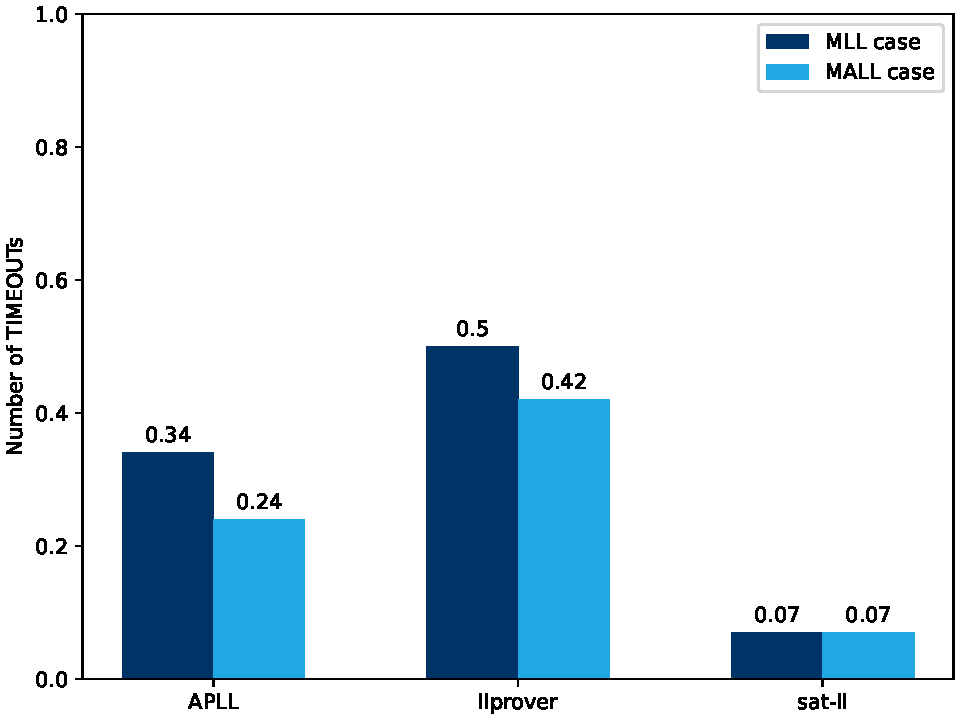
\includegraphics[scale=.4]{images/graph}
			\end{figure}
		\end{column}
	\end{columns}
\end{frame}
\begin{frame}{Risultati -- caso generale}
	Nel caso dei test esponenziali i risultati si livellano:
	\begin{table}[h!]
		\begin{subtable}{\textwidth}
			\centering
			{\footnotesize
			\begin{tabular}{ | l c c c c c c | }
				\hline
				\textbf{prover} & \textbf{timeouts} & \textbf{failures} & \textbf{successes} & \textbf{success rate} & \textbf{avg. (succ.)} & \textbf{avg. (tot.)} \\
				\hline
				\hline
				APLL     & $0$  & $17$ & $71$ & \color{darkbluestatale}{$\approx 0.80$} & \qty{0.035}{\second} & \qty{0.326}{\second} \\
				llprover & $20$ & $6$  & $62$ & \color{darkbluestatale}{$\approx 0.70$} & \qty{0.981}{\second} & \qty{2.179}{\second} \\
				sat-ll   & $5$  & $15$ & $68$ & \color{darkbluestatale}{$\approx 0.77$} & \qty{0.443}{\second} & \qty{0.496}{\second} \\
				\hline
			\end{tabular}
			}
			\caption{Output per KLE-cbv}
			\label{table:KLE-cbv}
		\end{subtable}
		\begin{subtable}{\textwidth}
			\centering
			{\footnotesize
			\begin{tabular}{ | l c c c c c c | }
				\hline
				\textbf{prover} & \textbf{timeouts} & \textbf{failures} & \textbf{successes} & \textbf{success rate} & \textbf{avg. (succ.)} & \textbf{avg. (tot.)} \\
				\hline
				\hline
				APLL     & $0$  & $16$ & $72$ & \color{darkbluestatale}{$\approx 0.80$} & \qty{0.037}{\second} & \qty{0.055}{\second} \\
				llprover & $20$ & $6$  & $62$ & \color{darkbluestatale}{$\approx 0.70$} & \qty{1.709}{\second} & \qty{3.253}{\second} \\
				sat-ll   & $4$  & $18$ & $66$ & \color{darkbluestatale}{$\approx 0.75$} & \qty{0.130}{\second} & \qty{0.185}{\second} \\
				\hline
			\end{tabular}
			}
			\caption{Output per KLE-cbn}
			\label{table:KLE-cbn}
		\end{subtable}
	\end{table}
\end{frame}

% ==================///==================///==================///
% ==================/// END PRESENTATION
% ==================///==================///==================///

\backmatter[notitle]

%=======================================================================

\end{document}
